% EmoH3 — IEEE ICASSP 2027 submission (4-page limit + references).
% Round 19 revision (reviewer-driven): 15-class judge, explicit success criterion,
% judge-validity sanity, protocol-sensitivity axes, statistical honesty.
% Compile:  tectonic paper_emoh3_icassp.tex   (IEEEtran conference, double-blind)
% Deadline (ICASSP 2027): 2026-09-16 (verify against the CFP before submitting).
\documentclass[conference]{IEEEtran}

% --- packages ---
\usepackage{graphicx}
\usepackage{booktabs}
\usepackage{amsmath,amssymb}
\usepackage{url}
\usepackage{xcolor}
\usepackage{textcomp}
\usepackage[colorlinks=true, linkcolor=blue, urlcolor=blue, citecolor=blue]{hyperref}

\title{Emotion-Control Evaluation Is Not Invariant: Judge, Option Order and
Judged Frame Span Flip 11--58\% of Verdicts on MiniMax H3}

\author{\IEEEauthorblockN{Anonymous}}

\begin{document}

\maketitle

\begin{abstract}
Portrait-reference (Ref2VA) video generators such as MiniMax H3 tend to lock the output to the
\emph{reference's} emotion, suppressing prompt-specified targets---most severely for negative and
subtle emotions. Studying this on MiniMax H3 (33B, joint video+audio, 8$\times$H100), we find that the
binding constraint is not the model but the measurement, and we quantify it along three orthogonal,
essentially free protocol choices. \textbf{(i) Judge}: across four open Qwen judges
(7B--32B, three generations \cite{qwen25vl2025,qwen3vl2025,qwen3827}) none validates on more than 1/17
taxonomy-relevant known emotions, none recognizes \emph{any} negative emotion, and on the same
clip-configs all four agree on only 23/77 (Fleiss $\kappa{=}0.38$; pairwise 41.6--71.6\%, each on its own common set), with
disagreement concentrated on \emph{whether} an emotion is present. \textbf{(ii) Option order}: merely
reversing the 15 answer options flips 17/88 and 10/88 verdicts on identical frames under greedy
decoding, while a duplicate run of one variant reproduces 88/88 word-identically. \textbf{(iii) Temporal coverage}---the largest \emph{within-judge}
axis and the only significant one (changing judge across capability tiers moves more, 58\%, but that is
not a free protocol choice in the same sense): our protocol, like much practice, judged 8 frames from the first second of each
5.2\,s clip; re-judging the whole clip changes 32/97, 32/97 and 34/97 verdicts under three judges (Cohen
$\kappa{=}0.48$--$0.57$), predominantly neutral$\rightarrow$committed, and raising target-hit rates in
three of six arm$\times$judge cells (base 8/34 to 16/34, exact McNemar $p{=}0.021$; LoRA 13/63 to 23/63
and 20/63 to 33/63, $p{=}0.002$, $0.001$) while leaving one unmoved (17/63 to 18/63 under
Qwen2.5-VL). On 14 externally labelled clips the wider span is also \emph{more accurate} in all six
judge$\times$rule comparisons. Prompted by this, we ran the matched experiment our earlier
comparison lacked---the base model regenerated on all 8 tasks $\times$ 2 seeds under identical inference
settings, 16 paired cells---and all four judges return a null result, the strongest of them scoring the
base \emph{higher} (base 4/16, 6/16, 9/16, 8/12 vs v3 6/16, 6/16, 8/16, 8/12; Fisher $p{\ge}0.70$). We therefore
\emph{retract} our task-level claim for a reference-conditioned LoRA and report it only as the case study
whose apparent result dissolves. What survives all four scorings is the mechanism---the LoRA suppresses
reference-emotion tracking (base 5/8, 4/8, 3/8, 4/8 vs v3 2/8 in each of those four conditions; 1/8 under a fifth,
Qwen2.5-VL)---and it is underpowered
($n{=}8$). Until judges are validated on the emotions they score and protocols fix temporal coverage,
reported emotion-control gains are not interpretable. All verdicts, frames and scripts are released.
\end{abstract}

\section{Introduction}
Character-consistent, emotion-controllable video generation is central to animation workflows:
given a character's portrait (reference) and a language instruction (``She smiles joyfully.''),
a generator should animate \emph{that} character \emph{in that state}. Recent portrait-reference
generators---e.g.\ MiniMax H3 Ref2VA~\cite{minimax2025}---preserve identity well, but show a strong
\emph{reference-emotion dominance}: output tends to reproduce the reference's expression, and
targets disagreeing with the reference are ignored, especially negative or subtle ones.

We ask whether this can be fixed on a single 8$\times$H100 node with an open 33B model, and find that the
binding constraint is measurement, not modelling. We make no claim of SOTA quality. Our contribution is
(a) a quantified, three-axis account of how unreliable emotion-control evaluation currently is, including
a directional systematic bias---short judged windows under-report emotion---that any such evaluation must
control; (b) the corresponding released corpus and toolkit: four judges $\times$ 88 clip-configs
$\times$ two frame spans $\times$ two option orders, with exact Fisher/McNemar analysis scripts; and
(c) a worked demonstration, on our own reference-conditioned LoRA, of how an apparent task-level result
dissolves when one of these axes is swept---which is why the LoRA appears here as a case study rather
than as a claimed improvement.
Findings: \textbf{(1)} evaluation is the weak link---every tested judge is partly blind, and verdicts
move with seed, taxonomy, judge, the \emph{order of the answer options}, and above all the
\emph{temporal span of the judged frames}, that last axis being systematic and significant;
\textbf{(2)} on a fully paired 8-task $\times$ 2-seed matrix the reference-conditioned LoRA shows no
task-level effect under any judge, so we retract that claim and keep only the mechanism, a measured
suppression of reference-emotion dominance; \textbf{(3)} frown-type targets are untestable with the
weakest judge (x04 becomes testable under newer ones); a resolution ablation rules out the layout
hypothesis.

\section{Related Work}
Open video diffusion transformers (CogVideoX~\cite{cogvideox2024}, HunyuanVideo~\cite{hunyuan2024},
Wan~\cite{wan2025}) and closed systems (Sora~\cite{sora2024}) drive progress; MiniMax
H3~\cite{minimax2025} is notable for joint video+audio with reference-image (Ref2VA) conditioning---the
model we study. Character-consistency methods condition on a reference via cross-attention adapters
(AnimateAnyone~\cite{animateanyone2023}, StableAnimator~\cite{stableanimator2024}) or image-prompt
adapters (IP-Adapter~\cite{ipadapter2023}); tuning-free, they preserve identity but control
\emph{emotion} weakly, since the reference encodes expression as well as identity. We use
LoRA~\cite{lora2021,dreambooth2022} for emotion \emph{behavior}. For automatic evaluation we adopt
Qwen2-VL-7B~\cite{qwen2vl2024} and, crucially, \emph{validate it} and \emph{sweep its inputs}---seed,
taxonomy, judge, option order and judged frame span---a methodological point that applies beyond our
task.

\section{Background: MiniMax H3 Ref2VA}
H3 is a 33B rectified-flow video+audio diffusion transformer. In Ref2VA mode the input is
$[\text{text}\mid\text{reference}\mid\text{target audio}\mid\text{target video}]$; the reference is
encoded by the video autoencoder, patched into conditioning rows and fed clean at pinned timestep
0.999, so it attends to every target token---making its emotion a strong prior. Our training
intervention mirrors this layout.

\section{Evaluation Protocol and Its Pitfalls}
\label{sec:proto}
\subsection{Protocol}
Eight emotion-transfer tasks, each a distinct character portrait plus a target-emotion prompt:
x01 neutral$\rightarrow$joyful, x02 neutral$\rightarrow$sad, x03 angry$\rightarrow$happy,
x04 joyful$\rightarrow$worried, x05 amused$\rightarrow$surprised, x06 anxious$\rightarrow$relieved,
x07 sad$\rightarrow$cheerful, x08 curious$\rightarrow$angry (prompts of the form ``She smiles
joyfully.'', ``She looks sad.''). We sample 8 frames (evenly over the first second of each 5.2\,s, 124-frame
clip---a coverage limitation we disclose and test in Sec.~\ref{sec:unstable}) and ask Qwen2-VL-7B
($\text{do\_sample}=$False) to classify emotion from a fixed \textbf{15-class taxonomy} with confidence. A task \emph{succeeds}
iff the judged emotion equals the target, with one stated synonym rule: joyful and cheerful map to
their in-taxonomy synonym \emph{happy}. The judge, frames, and seeds are all swept
(Sec.~\ref{sec:unstable}).



\subsection{Result 1: the evaluation is the weak link}
\label{sec:unstable}
We sweep five protocol axes. \textbf{(a) Judge conservatism:} across the 88 clip-configs the 15-class judge
emits only four words (neutral, happy, sad, surprised), never worried/relieved/angry, so x04/x06/x08 are
\emph{untestable} with it. \textbf{(b) Judge validity:} on the 17 portraits shared by all four
judges (Table~\ref{tab:judges}) it labels 1/17 correctly (4/17 leniently) and \emph{no} negative emotion
(0/5); 3/21 and 7/21 on its own set. Successes are lower bounds.
\textbf{(c) Judge choice:} verdicts flip with seed (v3 x02: neutral at s42, sad at s1234), frame count
(4/88 configs), taxonomy (12 vs 15 classes) and judge---Qwen2.5-VL-7B and Qwen3-VL-32B
\cite{qwen3vl2025} read the decisive v3 x02 clip as neutral:85 and worried:85 where Qwen2-VL says sad:80
and Qwen3.8-27B sad:82 (sad:80 in the 88-config log used for the agreement statistics; the
runs differ in confidence, not label). Across 88 configs and four judges, agreement is high \emph{within} a
capability tier (71.6\%, $\kappa{=}0.49$, for the two 7B models; 75.3\% on the 77-config four-judge
intersection; 68.8\%, $\kappa{=}0.63$, for the two newest, $n{=}77$) but 41.6--47.7\% \emph{across}
tiers, with only 23/77 configs unanimous (Fleiss $\kappa{=}0.38$; Qwen3.8-27B parses 77 rows). Raw
agreement is inflated by a shared neutral default: on the three-judge 88-config set, excluding configs both
call neutral leaves 33.8--45.7\%, yet where \emph{both} commit they agree 88--95\% (36.7--50.0\% and
87.9--100\% on the four-judge 77-config intersection)---a differing \emph{neutrality threshold}, not label
confusion (classes used 4/15, 6/15, 9/15, 9/15; Qwen2-VL calls 72\% of clips neutral). \textbf{(d) Option order:} reversing the 15 answer options---same judge, same
frames, greedy---flips 17/88 verdicts for Qwen2-VL (self-agreement 80.7\%, $\kappa{=}0.65$) and 10/88
for Qwen3-VL-32B (88.6\%, $\kappa{=}0.86$), whereas a duplicate run of the reversed variant reproduces 88/88
labels word-identically (one confidence differs): prompt sensitivity, not sampling noise. It lands on decision-relevant cells---base x01 flips
neutral$\rightarrow$happy and Qwen3-VL-32B's dissent on the decisive v3 x02 clip flips
worried$\rightarrow$sad.

\textbf{(e) Temporal frame coverage---the largest within-judge effect, and the only significant one.} Our 8 judged
frames, like much reported practice, were sampled over the first second of each 5.2\,s (124-frame,
24\,fps) clip: 19\% of the clip, and precisely the part still closest to the reference. Re-extracting 8
frames across the \emph{whole} clip and changing nothing else flips \textbf{32/97} verdicts for Qwen2-VL
(self-agreement 67.0\%, $\kappa{=}0.48$), \textbf{32/97} for Qwen2.5-VL (67.0\%, $\kappa{=}0.48$) and
\textbf{34/97} for Qwen3-VL-32B (64.9\%, $\kappa{=}0.57$)---a third of all verdicts, under every judge we
re-scored. The flips are directional, not noisy: 28 of Qwen2-VL's 32 are neutral$\rightarrow$committed and
non-neutral verdicts rise (31/97 to 56/97; 73 to 85 for Qwen3-VL-32B), though Qwen3-VL-32B's flips are
mostly committed$\rightarrow$committed (20/34). We report all six arm$\times$judge hit-rate cells, because
three are significant and one does not move at all: base 8/34$\rightarrow$16/34 (exact McNemar
$p{=}0.021$), 12/34$\rightarrow$16/34 and 17/34$\rightarrow$22/34 ($p{=}0.125$ both); LoRA
13/63$\rightarrow$23/63 ($p{=}0.002$) and 20/63$\rightarrow$33/63 ($p{=}0.001$), but
17/63$\rightarrow$18/63 under Qwen2.5-VL ($p{=}1.00$). Two of the six survive Bonferroni correction
($\alpha/6$). The flat cell is not an inconvenience but an instance of the thesis: the frame-span effect
is itself judge-dependent. These are the only significant \emph{model-side} effects we obtain. Emotion in
these clips is largely \emph{absent at the start and expressed later}, so judging a clip's opening
systematically under-measures emotion control; the consequences for our own claims appear in Finding~B.
Is the longer window \emph{better} or merely different? It is
\textbf{more accurate against external labels}. The 14 source clips in our training manifest come from the same
production batch as the portraits above and carry that batch's intended expression in their filenames, so
they need no annotation of ours. Judging their first second recovers the label 0/14, 0/14, 5/14 (strict;
4/14, 3/14, 7/14 leniently); judging the whole clip recovers 3/14, 4/14, 9/14 (8/14, 9/14, 11/14). All six comparisons improve, and
of 25 clips whose correctness changes, \emph{all 25} favour the whole clip and none the opening (exact
McNemar $p{=}0.031$ at best, $0.125$ typical). Inter-judge reliability agrees more weakly: over the 97
clips all three pairs move the same way but only Qwen2-VL vs Qwen3-VL-32B significantly
($\kappa\,0.348{\rightarrow}0.462$, paired bootstrap $P{=}0.035$; others $+0.011$, $+0.001$).
The primary protocol remains 8 frames over the first second, for comparability with earlier rounds, with
full-span re-scoring reported alongside.

\textbf{Result 2: the baseline's apparent weakness is largely an artifact of the scoring.} Under Qwen2-VL
the base succeeds on x03 but never on negative targets and x01/x07 are neutral, consistent with
reference-emotion dominance (Sec.~\ref{sec:mech}); yet stronger judges credit the base on 3/4 matched
tasks, Qwen2-VL itself credits x01 once the option list is reversed, and under full-clip scoring x01 and
x07 both flip to happy---i.e.\ every ``failure'' we relied on is recoverable by a protocol change alone.

\section{Method: Reference-Conditioned LoRA (case study)}
We hypothesize reference-emotion dominance persists because training never conditions on the reference:
a naive LoRA learns a \emph{reference-agnostic} prompt$\rightarrow$emotion mapping, so at inference the
reference wins. We teach the model to \emph{use} the reference by conditioning the training forward on
it in the exact Ref2VA layout: the cache builder encodes each reference image
with the video autoencoder exactly as at inference (cover-resize, spatial encode, sample posterior seed
42, float16, normalize, patchify); packing is
$[\text{text}\mid\text{reference}\mid\text{target audio}\mid\text{target video}]$, reference rows are fed
\emph{clean} at $t{=}0.999$, loss only on target rows, sequences grow 537$\rightarrow{\approx}$602 rows.
Data: 22 clips on one 8$\times$H100 node---10 \emph{preservation} clips (reference and target share the
emotion) and 12 \emph{cross-emotion} pairs for one character (reference emotion $A$, target $B\neq A$),
the ``prompt overrides reference'' supervision. LoRA rank 16/alpha 32, 900 steps. The 8 eval tasks use 7
\emph{different} references; x01/x02 use an actor \emph{absent} from training. Our v1/v2 ladder (both
reference-agnostic) is the ablated baseline; external methods do not transfer to this base model.



\section{Experiments}
\label{sec:setup}
\subsection{Setup}
Models: base; v1 (9 clips, 300 steps); v2 (18 clips, 600 steps); \textbf{v3 (reference-conditioned,
22 clips, 256$^2$, 900 steps)}; v4 (same data, 768$^2$, 900 steps)---v3/v4 isolate training
resolution. Inference 768$\times$768$\times$124, 16 steps, seeds 42/1234 (and 999/sweep for key
tasks), 8-frame judge. Success = judged emotion == target (synonym rule of Sec.~\ref{sec:proto}); the full per-configuration success matrix is released with the logs.

\subsection{Main results}
Table~\ref{tab:sensitivity} is the paper's main result; Fig.~\ref{fig:qual} shows representative frames.

\begin{figure}[!t]
\centering
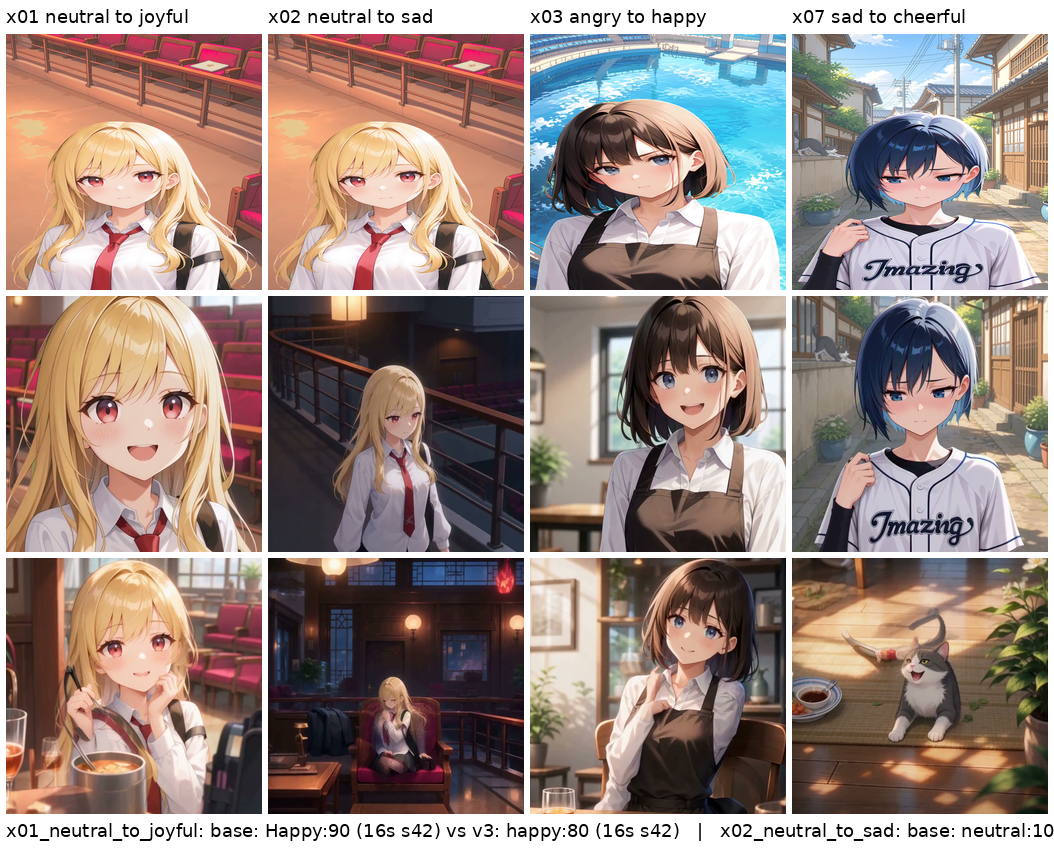
\includegraphics[width=0.93\columnwidth]{paper_figure1.png}
\caption{Representative base-vs-v3 frames with 15-class verdicts under the primary protocol. The
neutral$\rightarrow$sad row is the cell whose verdict does not survive full-clip re-scoring.}
\label{fig:qual}
\end{figure}

\begin{table}[!t]
\centering\footnotesize
\caption{\textbf{Protocol sensitivity is the main result.} Each row changes one scoring choice and
nothing else---same clips, same 15-class forced choice, greedy decoding---and reports how many verdicts
move. Frame span is the largest axis that keeps the judge fixed, and the only significant one; a
duplicate run of an unchanged
configuration is the noise floor.}
\label{tab:sensitivity}
\begin{tabular}{@{}llcc@{}}
\toprule
Axis changed & Judge & Agr. & Flips \\
\midrule
nothing (duplicate) & Qwen2-VL & 100\% & 0/88 \\
option order & Qwen2-VL & 80.7\% & 17/88 \\
option order & Qwen3-VL-32B & 88.6\% & 10/88 \\
frame span 1$\rightarrow$5.2\,s & Qwen2-VL & \textbf{67.0\%} & \textbf{32/97} \\
frame span 1$\rightarrow$5.2\,s & Qwen2.5-VL & \textbf{67.0\%} & \textbf{32/97} \\
frame span 1$\rightarrow$5.2\,s & Qwen3-VL-32B & \textbf{64.9\%} & \textbf{34/97} \\
judge, same tier & 2-VL vs 2.5-VL & 71.6\% & 25/88 \\
judge, across tiers & 2-VL vs 3-VL-32B & 42.0\% & 51/88 \\
judge, all four & unanimous & 23/77 & --- \\
\bottomrule
\end{tabular}
\end{table}



\begin{table}[!t]
\centering\footnotesize
\caption{Four open VLM judges, same 15-class protocol and frames, on the 17 known-emotion portraits
whose labels are inside the taxonomy (identical set for all four). Strict = exact match; lenient applies
the synonym rule. None passes, and \emph{no judge recognizes any negative emotion} (0/5 for all four):
on a clear crying portrait the dissenters answer ``surprised'' and the corroborating Qwen3.8-27B
answers ``fearful''. Base x02 is neutral under all four; v3 x02 is sad under Qwen2-VL and Qwen3.8-27B.
Verdicts parsed as the last WORD:SCORE of each raw response (released).}
\label{tab:judges}
\begin{tabular}{@{}lccccc@{}}
\toprule
Judge & s. strict & s. len. & v3 x02 & base x02\\
\midrule
Qwen2-VL-7B & 1/17 & 4/17 & \textbf{sad 80} & neutral 50\\
Qwen2.5-VL-7B & 0/17 & 5/17 & neutral 85 & neutral 95\\
Qwen3-VL-32B & 1/17 & 6/17 & worried 85 & neutral 95\\
Qwen3.8-27B & 0/17 & 7/17 & \textbf{sad 82} & neutral 78\\
\bottomrule
\end{tabular}
\end{table}

\textbf{Finding A --- the decisive cell is scoring-dependent, and its control does not hold.}
Task x02 (neutral$\rightarrow$sad) was our only negative target ever scored as hit: v3 sad (80) at one of
eight seeds against 0/7 for base on the unmatched set---not significant (Fisher $p{=}1.00$), one
generation per model, and it does not survive matching, since Qwen3-VL-32B judges base x02 at seed 42
\emph{sad} (Finding~B). Its verdict moves along every axis at once (Table~\ref{tab:judges}): Qwen2-VL says
sad:80 and Qwen3.8-27B \cite{qwen3827} sad:85/82, Qwen3-VL-32B dissents (worried:85) but flips to
\emph{sad} when the option list is reversed, and an 8-frame montage flips v3 to neutral. Both dissenters
mislabel a clear crying portrait ``surprised'' while Qwen3.8-27B reads it fearful:85---the static check
fails for \emph{every} judge (0/5). We keep x02 only as an illustration of the thesis.

\textbf{Finding B --- we retract our task-level claim: a matched experiment shows no effect.} Our earlier
comparison was not task-matched: the base model had 16-step clips for only 4 of the 8 tasks
(x01/x02/x03/x07), so any aggregate over the 88-config pool---which also contains reference-swap probes,
an x02 seed sweep and non-16-step rows---mixes task composition into the ``success rate.'' We therefore
regenerated the base model on \textbf{all 8 tasks at both seeds} under inference settings identical to the
v3 evaluation, giving a fully paired 16-cell matrix, and judged it with the same protocol
(Table~\ref{tab:retract}). All four judges return a null result, and the strongest scores the base
\emph{higher}: base 4/16 vs v3 6/16 (Qwen2-VL, Fisher $p{=}0.70$, paired McNemar $p{=}0.69$), 6/16 vs
6/16 (Qwen2.5-VL, $p{=}1.00$), 9/16 vs 8/16 (Qwen3-VL-32B, $p{=}1.00$) and 8/12 vs 8/12 (Qwen3.8-27B, on
the 12 cells it parses, $p{=}1.00$). Two cells of that matrix
independently destroy the premises our earlier reading rested on, under the primary protocol and with no
appeal to frame span: \textbf{base x02 at seed 42 is judged sad} by Qwen3-VL-32B, so ``the base never
expresses sad'' is false; and \textbf{base x08 at seed 1234 is judged angry} by two judges, so the
frown-type boundary is not a base-model wall either. Re-scoring the older matched clips over the full clip
(Sec.~\ref{sec:unstable}(e)) points the same way---both arms end level---but that argument is now
secondary: the matched experiment measures the effect directly and finds none. We therefore retract the task-level claim: the reference-conditioned
LoRA shows \textbf{no measurable task-level improvement} in emotion control, and the appearance of one
came from an unmatched comparison scored over the opening second of each clip. What the intervention does
change is the mechanism (Finding~D).

\textbf{Finding C --- frown-type targets are untestable only with the weakest judge.} Worried (x04) and
angry (x08) are \emph{never emitted} by Qwen2-VL (4/15 classes), so their failure is unattributable with
it. Qwen3-VL-32B (9/15) and Qwen3.8-27B judge v3 x04 \emph{worried} (85, 80), and x08 is reached by the
\emph{base} model (s1234, angry under two judges). Both also read a known-sad portrait as worried: this is
a boundary on our \emph{evaluation}.

\textbf{Finding D --- direct evidence for reference-emotion dominance and its suppression.}
\label{sec:mech}
Table~\ref{tab:mechanism} holds the prompt fixed (``She looks sad.'') and varies the reference emotion
(four portraits, both seeds). The base output tracks the \emph{reference} (sad 2/2, surprised 2/2, joyful
1/2), confirming the root cause; v3 is decoupled (mostly neutral). Unlike the task-level gain,
\emph{this is the only claim that survives every scoring we tried}: tracking falls from 5/8, 4/8, 4/8
(base) to 2/8, 1/8, 2/8 (v3) under the three judges, and holds under full-clip re-scoring (3/8, 4/8 vs
2/8, 2/8). Under $\ge$2-of-3 consensus it is base 4/8 vs v3 2/8, both discordant pairs favouring
suppression (exact McNemar $p{=}0.50$), so this is a consistent \emph{direction}, not an established
effect, and is partly indistinguishable from regression toward neutral.

\begin{table}[!t]
\centering\footnotesize
\caption{The retraction in one table. \emph{Top}: the fully paired matrix---base regenerated on all 8
tasks $\times$ 2 seeds under the v3 inference settings, same 15-class protocol, 16 paired cells. All four
judges are null and the strongest scores the base higher. \emph{Bottom}: the older 4-task matched set
re-scored over the whole clip instead of the first second; both arms end level. Two cells of the paired
matrix also falsify the premises the earlier reading used: base x02 (s42) is judged \emph{sad} and base
x08 (s1234) \emph{angry}. $^{*}$Qwen3.8-27B parses 12 of the 16 cells.}
\label{tab:retract}
\begin{tabular}{@{}lccc@{}}
\toprule
Paired 8$\times$2 matrix & base & v3 & Fisher / McN. $p$\\
\midrule
Qwen2-VL-7B      & 4/16 & 6/16 & 0.70 / 0.69\\
Qwen2.5-VL-7B    & 6/16 & 6/16 & 1.00 / 1.00\\
Qwen3-VL-32B     & \textbf{9/16} & 8/16 & 1.00 / 1.00\\
Qwen3.8-27B$^{*}$ & 8/12 & 8/12 & 1.00 / 1.00\\
\midrule
4-task set, frames judged & base & v3 & judge\\
\midrule
first 1\,s (primary)  & 1/4 & 2/4 & Qwen2-VL\\
whole clip (5.2\,s)   & 3/4 & 3/4 & Qwen2-VL\\
1\,s \emph{and} whole clip & 3/4 & 3/4 & Qwen3-VL-32B\\
\bottomrule
\end{tabular}
\end{table}

\begin{table}[!t]
\centering\footnotesize
\caption{Reference-swap, prompt fixed ``She looks sad.'' (15-class, 16 steps, 8 frames). Base tracks the
reference; v3 decouples (mostly neutral); angry is never emitted as angry.}
\label{tab:mechanism}
\begin{tabular}{@{}lccccc@{}}
\toprule
Ref & base & base & v3 & v3\\
 & s42 & s1234 & s42 & s1234\\
\midrule
angry & sad 80 & neut 50 & neut 100 & neut 50\\
joyful & neut 50 & \textbf{hap 80} & neut 50 & neut 100\\
sad & \textbf{sad 80} & \textbf{sad 80} & sad 80 & sad 80\\
surprised & \textbf{surp 80} & \textbf{surp 100} & neut 50 & neut 100\\
\bottomrule
\end{tabular}
\end{table}

\textbf{Ablation (resolution).} v4 (768$^2$) is \emph{worse} than v3 (256$^2$) with \emph{lower}
training loss (0.30 vs 0.45), consistent with overfitting: resolution is not the bottleneck.

\section{Limitations and Conclusion}
(i) All four judges fail the validity check (1/17, 0/17, 1/17, 0/17; 0/5 negative), so every count is
instrument-limited, and our accuracy check uses the source batch's intended labels rather than our own
annotation of these clips. (ii) Small $n$: 16 paired cells, 14 labelled clips, 8 mechanism conditions, 97
re-scored clips. (iii) The reference-swap test uses the training character; audio is judged video-only;
external baselines do not transfer to this base model.

\textbf{Conclusion.} Emotion-control evaluation here is not invariant to three free protocol choices:
judge identity (23/77 unanimous, none validated), option order (up to 19\% of verdicts flip) and judged
frame span (up to 35\%, and the wider span recovers externally labelled emotions better). Following that
axis to a matched experiment retracted our own task-level claim: single-protocol gains are not
interpretable.

\bibliographystyle{IEEEtran}
\begin{thebibliography}{14}

\bibitem{minimax2025} MiniMax, ``MiniMax H3: open-source 33B video and audio model,'' \emph{arXiv:2507.12572}, 2025.
\bibitem{cogvideox2024} Z.~Yang \emph{et al.}, ``CogVideoX: text-to-video diffusion models with an expert transformer,'' \emph{arXiv:2408.06072}, 2024.
\bibitem{hunyuan2024} Tencent, ``HunyuanVideo: a systematic framework for large video generative models,'' \emph{arXiv:2412.03603}, 2024.
\bibitem{wan2025} Wan Team, ``Wan: open and advanced large-scale video generative models,'' \emph{arXiv:2503.20314}, 2025.
\bibitem{sora2024} OpenAI, ``Video generation models as world simulators (Sora),'' 2024.
\bibitem{animateanyone2023} A.~Hu, ``Animate Anyone: Consistent and controllable image-to-video synthesis for character animation,'' \emph{arXiv:2311.17117}, 2023.
\bibitem{stableanimator2024} H.~Tian \emph{et al.}, ``StableAnimator: High-quality identity-preserving human image animation,'' \emph{arXiv:2411.17697}, 2024.
\bibitem{ipadapter2023} H.~Ye \emph{et al.}, ``IP-Adapter: Text compatible image prompt adapter for text-to-image diffusion models,'' \emph{arXiv:2308.06721}, 2023.
\bibitem{lora2021} E.~Hu \emph{et al.}, ``LoRA: Low-rank adaptation of large language models,'' \emph{arXiv:2106.09685}, 2021.
\bibitem{dreambooth2022} N.~Ruiz \emph{et al.}, ``DreamBooth: Fine tuning text-to-image diffusion models for subject-driven generation,'' \emph{arXiv:2208.12242}, 2022.
\bibitem{qwen2vl2024} P.~Wang \emph{et al.}, ``Qwen2-VL: Enhancing vision-language models' perception of the world at any resolution,'' \emph{arXiv:2409.12191}, 2024.
\bibitem{qwen25vl2025} Qwen~Team, ``Qwen2.5-VL technical report,'' \emph{arXiv:2502.13923}, 2025.
\bibitem{qwen3vl2025} Qwen~Team, ``Qwen3-VL-32B-Instruct,'' \emph{model card}, 2025, \url{https://huggingface.co/Qwen/Qwen3-VL-32B-Instruct}.
\bibitem{qwen3827} Qwen~Team, ``Qwen3.8-27B,'' \emph{model card}, 2026, \url{https://huggingface.co/Qwen/Qwen3.8-27B}.
\end{thebibliography}

\end{document}
